\documentclass[10pt,a4paper]{article}
\usepackage[utf8]{inputenc}
\usepackage{amsmath}
\usepackage{dsfont}
\usepackage{amsfonts}
\usepackage{amssymb}
\usepackage{graphicx}

\author{Leander van Beek}
\title{Problem 7 | 10001st prime}

\newcommand{\desda}{\textbf{if and only if} }

\begin{document}

\maketitle

\textbf{Problem:} By listing the first six prime numbers: 2, 3, 5, 7, 11, and 13, we can see that the 6th prime is 13.\\

What is the 10 001st prime number?\\


\vspace{0.5cm}
\hrule
\vspace{0.5cm}

To solve this problem we will use the sieve of Eratosthenes. This is a simple algorithm do find prime numbers in a list. An upper bound for the list is required. Write out all numbers from $1$ to $N$, $N$ being the largest number that will be scanned. Then, start crossing out every 2nd number from the list except the first one - two itself. Repeat this process for every third number, every fourth number, etcetera. Stop when you reach $N/2$ as numbers larger than this will not be divisible by anything other than themselves if they have not yet been crossed out, making them prime by definition. All numbers that have not been crossed out, are prime numbers.\\

\begin{figure}[h]
\centering
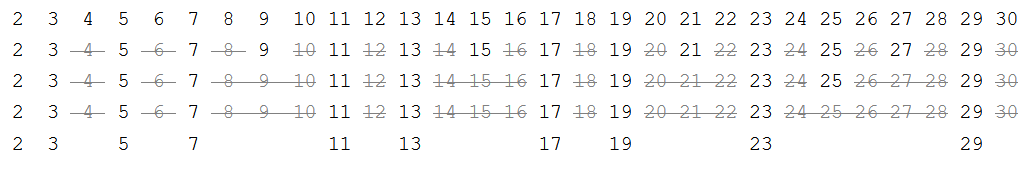
\includegraphics[width=0.85\linewidth]{crossings.png}
\end{figure}

A small problem here is to determine $N$ - the number up to where to scan. To determine N, the prime number theorem can be used. The prime number theorem predicts the density of primes along the real axis as $p_n ~ n \log(n)$. Multiplying this factor with some number slightly larger than 1 to have some margin, setting $N$ to be $1.5 n \log(n)$ in our case to $1.5 * 10001 * \log(10001)$ is a safe bet.\\

Indeed, checking the amount of remaining primes after the checking, there are plenty to spare. Selecting the $10001$st, it turns out to be 104743.


\end{document}